\documentclass[14pt,a4paper,report]{report}
\usepackage[a4paper, mag=1000, left=2.5cm, right=1cm, top=2cm, bottom=2cm, headsep=0.7cm, footskip=1cm]{geometry}
\usepackage[utf8]{inputenc}
\usepackage[english,russian]{babel}
\usepackage{indentfirst}
\usepackage[dvipsnames]{xcolor}
\usepackage[colorlinks]{hyperref}
\usepackage{listings} 
\usepackage{fancyhdr}
\usepackage{caption}
\usepackage{amsmath}
\usepackage{latexsym}
\usepackage{graphicx}
\usepackage{amsmath}
\hypersetup{
	colorlinks = true,
	linkcolor  = black
}

\usepackage{titlesec}
\titleformat{\chapter}
{\Large\bfseries} % format
{}                % label
{0pt}             % sep
{\huge}           % before-code


\DeclareCaptionFont{white}{\color{white}} 

% Listing description
\usepackage{listings} 
\DeclareCaptionFormat{listing}{\colorbox{gray}{\parbox{\textwidth}{#1#2#3}}}
\captionsetup[lstlisting]{format=listing,labelfont=white,textfont=white}
\lstset{ 
	% Listing settings
	inputencoding = utf8,			
	extendedchars = \true, 
	keepspaces = true, 			  	 % Поддержка кириллицы и пробелов в комментариях
	language = Matlab,            	 	 % Язык программирования (для подсветки)
	basicstyle = \small\sffamily, 	 % Размер и начертание шрифта для подсветки кода
	numbers = left,               	 % Где поставить нумерацию строк (слева\справа)
	numberstyle = \tiny,          	 % Размер шрифта для номеров строк
	stepnumber = 1,               	 % Размер шага между двумя номерами строк
	numbersep = 5pt,              	 % Как далеко отстоят номера строк от подсвечиваемого кода
	backgroundcolor = \color{white}, % Цвет фона подсветки - используем \usepackage{color}
	showspaces = false,           	 % Показывать или нет пробелы специальными отступами
	showstringspaces = false,    	 % Показывать или нет пробелы в строках
	showtabs = false,           	 % Показывать или нет табуляцию в строках
	frame = single,              	 % Рисовать рамку вокруг кода
	tabsize = 2,                  	 % Размер табуляции по умолчанию равен 2 пробелам
	captionpos = t,             	 % Позиция заголовка вверху [t] или внизу [b] 
	breaklines = true,           	 % Автоматически переносить строки (да\нет)
	breakatwhitespace = false,   	 % Переносить строки только если есть пробел
	escapeinside = {\%*}{*)}      	 % Если нужно добавить комментарии в коде
}

\begin{document}

\def\contentsname{Содержание}

% Titlepage
\begin{titlepage}
	\begin{center}
		\textsc{Санкт-Петербургский Политехнический 
			Университет Петра Великого\\[5mm]
			Кафедра компьютерных систем и программных технологий}
		
		\vfill
		
		\textbf{Отчёт по лабораторной работе №2\\[3mm]
			Курс: «Теория автоматического управления»\\[3mm]
			Тема: «Изучение различных форм представления системы»\\[35mm]
			}
	\end{center}
	
	\hfill
	\begin{minipage}{.5\textwidth}
		Выполнил студент:\\[2mm] 
		Волкова Мария Дмитриевна\\
		Группа: 43501/3\\[5mm]
		
		Проверил:\\[2mm] 
		Нестеров Сергей Александрович
	\end{minipage}
	\vfill
	\begin{center}
		Санкт-Петербург\\ \the\year\ г.
	\end{center}
\end{titlepage}

% Contents
\tableofcontents


п\chapter{Лабораторная работа №2}

\section{Цель работы}

Получить навыки работы с моделями ВСВ и каноническими представлениями.

\section{Программа работы}

\begin{itemize}
	\item Представить систему в трех канонических формах.
	\item Получить структурные схемы для каждой формы.
	\item Получить матрицы управляемости и матрицы преобразования.
	\item Проверить систему на устойчивость, наблюдаемость и управляемость.
\end{itemize}

\section{Индивидуальное задание}

$
\\
y''+2y'=0.75u'+0.75u, y(0)=0, y'(0)=0, u=1(t)\\\\
W(p)=\frac{y}{u}=\frac{0.75}{p^2+2p+0.75}
$

\newpage
\section{Ход работы}

\subsection{Построение канонических форм}

\subsubsection{Нормальная форма управления}

\begin{equation*}
\text{$W(p)=\frac{y}{u}=\frac{0.75}{p^2+2p+0.75}=\frac{y}{u}$}
\end{equation*}

\begin{equation*}
\text{$\frac{y}{0.75}=\frac{u}{p^2+2p+0.75}=x_1$}
\Longrightarrow
\begin{cases}
	\text{$u=x_1(p^2+2p+0.75)$} \\
	\text{$y=x_1(0.75)$}
\end{cases}
\end{equation*}

\begin{equation*}
\begin{cases}
	\text{$px_1=x_2$} \\
	\text{$px_2=u-2x_2-0.75x_1$}\\
	\text{$y=0.75x_1$}
\end{cases}
\end{equation*}

\begin{equation*}
\text{$A=$}
\text{$
\begin{bmatrix}
0 & 1 \\
-0.75 & -2 \\
\end{bmatrix}
$}
\text{$, B=$}
\text{$
\begin{bmatrix}
0 \\
1 \\
\end{bmatrix}
$}
\text{$, C=$}
\text{$
\begin{bmatrix}
0.75 & 0 \\
\end{bmatrix}
$}
\end{equation*}

Проверим корректность полученных матриц $A, B, C$:

\begin{equation*}
\text{$det(A-\lambda)=0$}
\Longrightarrow
\text{$-\lambda(-2-\lambda)=0$}
\Longrightarrow
\begin{cases}
	\text{$\lambda_1=0$} \\
	\text{$\lambda_2=-2$}
\end{cases}
\end{equation*}

Собственные числа совпадают с собственными числами матриц в нормальной форме наблюдения и канонической форме, что свидетельствует о корректности полученных матриц  $A, B, C$.

\begin{equation*}
\text{$W(p)=C(pE-A)^{-1}B=
\begin{bmatrix}
0.75 & 0 \\
\end{bmatrix}
\begin{bmatrix}
p & 1 \\
0.75 & p+2\\
\end{bmatrix}^{-1}
\begin{bmatrix}
0 \\
1 \\
\end{bmatrix}=
\begin{bmatrix}
0.75 & 0 \\
\end{bmatrix}
\begin{bmatrix}
\frac{1}{p} & \frac{1}{p^2+2p} \\
0.75 & \frac{1}{p+2}\\
\end{bmatrix}
\begin{bmatrix}
0 \\
1 \\
\end{bmatrix}=
$}
\end{equation*}

\begin{equation*}
\text{$=\begin{bmatrix}
	\frac{0.75}{p} & \frac{0.75}{p^2+2p+0.75} \\
	\end{bmatrix}\begin{bmatrix}
	0 \\
	1 \\
	\end{bmatrix}=\frac{y}{u}=\frac{0.75}{p^2+2p+0.75}
	$}
\end{equation*}

Передаточная функция, полученная в результате преобразования $W(p)=C(pE-A)^{-1}B$, полностью совпадает с исходной, что свидетельствует о корректности полученных матриц  $A, B, C$. 

\begin{figure}[h!]
	\centering
	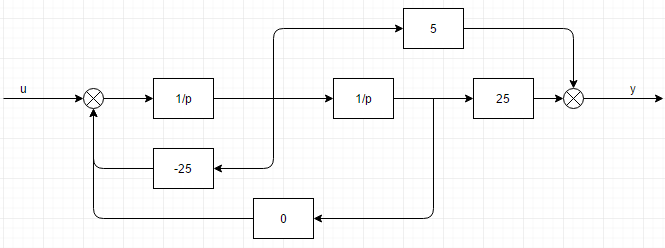
\includegraphics[scale = 0.55]{images/nfu.png}
	\caption{Структурная схема НФУ}
	\label{image:1}
\end{figure}
\newpage
\subsubsection{Нормальная форма наблюдения}

\begin{equation*}
\text{$W(p)=\frac{y}{u}=\frac{0.75}{p^2+2p+0.75}=\frac{y}{u}$}
\Longrightarrow
\text{$(0.75)u=(p^2+2p+0.75)y$}
\Longrightarrow
\end{equation*}

\begin{equation*}
\Longrightarrow
\text{$p^2y+2py+0.75y-0.75u=0$}
\Longrightarrow
\text{$p(py+2y)+(0.75y-0.75u)=0$}
\end{equation*}

\begin{equation*}
\begin{cases}
	\text{$x_1=py+2y$} \\
	\text{$px_1=0.75y-0.75u$} \\
\end{cases}
\Longrightarrow
\begin{cases}
	\text{$x_2=y$}\\
	\text{$x_1=px_2+2	x_2$} \\
	\text{$px_1=0.75y-0.75u$} \\
\end{cases}
\Longrightarrow
\begin{cases}
	\text{$px_1=25u$} \\
	\text{$px_2=x_1-2x_2$} \\
	\text{$y=x_2$}
\end{cases}
\end{equation*}

\begin{equation*}
\text{$A=$}
\text{$
	\begin{bmatrix}
	0 & -0.75 \\
	1 & -2 \\
	\end{bmatrix}
	$}
\text{$, B=$}
\text{$
	\begin{bmatrix}
	0.75 \\
	0 \\
	\end{bmatrix}
	$}
\text{$, C=$}
\text{$
	\begin{bmatrix}
	0 & 1 \\
	\end{bmatrix}
	$}
\end{equation*}

Проверим корректность полученных матриц $A, B, C$:

\begin{equation*}
\text{$det(A-\lambda)=0$}
\Longrightarrow
\text{$-\lambda(-2-\lambda)=0$}
\Longrightarrow
\begin{cases}
	\text{$\lambda_1=0$} \\
	\text{$\lambda_2=-2$}
\end{cases}
\end{equation*}

Собственные числа совпадают с собственными числами матриц в нормальной форме наблюдения и канонической форме, что свидетельствует о корректности полученных матриц  $A, B, C$.

\begin{equation*}
\text{$W(p)=C(pE-A)^{-1}B=
\begin{bmatrix}
0 & 1 \\
\end{bmatrix}
\begin{bmatrix}
p & -0.75 \\
1 & p+2\\
\end{bmatrix}^{-1}
\begin{bmatrix}
0.75 \\
0 \\
\end{bmatrix}=\begin{bmatrix}
0.75 & 0 \\
\end{bmatrix}
\begin{bmatrix}
\frac{1}{p} & \frac{0.75}{p+0.75} \\
\frac{1}{p^2+2p} & \frac{1}{p+2}\\
\end{bmatrix}
\begin{bmatrix}
0\\
1 \\
\end{bmatrix}=
$}
\end{equation*}

\begin{equation*}
\text{$=\begin{bmatrix}
\frac{0.75}{p^2+2p+0.75} & \frac{p}{p^2+25p} \\
\end{bmatrix}\begin{bmatrix}
0\\
1 \\
\end{bmatrix}=\frac{0.75}{p^2+2p+0.75}
$}
\end{equation*}

Передаточная функция, полученная в результате преобразования $W(p)=C(pE-A)^{-1}B$, полностью совпадает с исходной, что свидетельствует о корректности полученных матриц  $A, B, C$. 


\begin{figure}[h!]
	\centering
	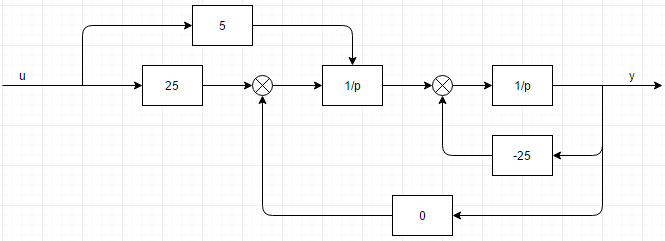
\includegraphics[scale = 0.9]{images/nfn.png}
	\caption{Структурная схема НФН}
	\label{image:2}
\end{figure}
\newpage
\subsubsection{Каноническая форма}

\begin{equation*}
\text{$W(p)=\frac{y}{u}=\frac{0.75}{p^2+2p+0.75}=\frac{5p+25}{p(p+25)}=\frac{1}{p}+\frac{4}{p+25}=\frac{y}{u}$}
\end{equation*}

\begin{equation*}
\begin{cases}
	\text{$\frac{x_1}{u}=\frac{1}{p}$} \\
	\text{$\frac{x_2}{u}=\frac{4}{p+25}$} \\
	\text{$y=x_1+x_2$}
\end{cases}
\Longrightarrow
\begin{cases}
\text{$px_1=u$} \\
\text{$px_2=-25x_2+4u$} \\
\text{$y=x_1+x_2$}
\end{cases}
\end{equation*}

\begin{equation*}
\text{$A=$}
\text{$
	\begin{bmatrix}
	0 & 0 \\
	0 & -25 \\
	\end{bmatrix}
	$}
\text{$, B=$}
\text{$
	\begin{bmatrix}
	1 \\
	4 \\
	\end{bmatrix}
	$}
\text{$, C=$}
\text{$
	\begin{bmatrix}
	1 & 1 \\
	\end{bmatrix}
	$}
\end{equation*}

Проверим корректность полученных матриц $A, B, C$:

\begin{equation*}
\text{$det(A-\lambda)=0$}
\Longrightarrow
\text{$-\lambda(-2-\lambda)=0$}
\Longrightarrow
\begin{cases}
	\text{$\lambda_1=0$} \\
	\text{$\lambda_2=-2$}
\end{cases}
\end{equation*}

Собственные числа совпадают с собственными числами матриц в нормальной форме управления и нормальной форме наблюдения, что свидетельствует о корректности полученных матриц  $A, B, C$

\begin{equation*}
\text{$W(p)=C(pE-A)^{-1}B=
	\begin{bmatrix}
	1 & 1 \\
	\end{bmatrix}
	\begin{bmatrix}
	p & 0 \\
	0 & p+25\\
	\end{bmatrix}^{-1}
	\begin{bmatrix}
	1 \\
	4 \\
	\end{bmatrix}=
	\begin{bmatrix}
	1 & 1 \\
	\end{bmatrix}
	\begin{bmatrix}
	\frac{1}{p} & 0 \\
	0 & \frac{1}{p+25}\\
	\end{bmatrix}
	\begin{bmatrix}
	1 \\
	4 \\
	\end{bmatrix}=
	$}
\end{equation*}

\begin{equation*}
\text{$=\begin{bmatrix}
	\frac{p+25}{p^2+25p} & \frac{p}{p^2+25p} \\
	\end{bmatrix}\begin{bmatrix}
	1 \\
	4 \\
	\end{bmatrix}=\frac{5p+25}{p^2+25p}
	$}
\end{equation*}

Передаточная функция, полученная в результате преобразования $W(p)=C(pE-A)^{-1}B$, полностью совпадает с исходной, что свидетельствует о корректности полученных матриц  $A, B, C$. 


\begin{figure}[h!]
	\centering
	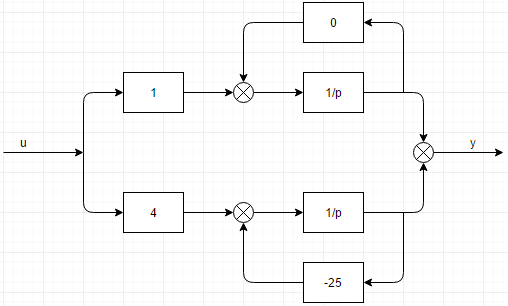
\includegraphics[scale = 0.9]{images/kf.png}
	\caption{Структурная схема КФ}
	\label{image:3}
\end{figure}


\newpage
\section{Вывод}


Модель ВСВ весьма гибкая, так как помимо трех канонических форм, рассмотренных в работе существу- ют произвольные формы, которые иногда могут быть полезны.
Отличия между каноническими формами наиболее явно проявляются на структурных схемах. Система, представленная в форме управления, имеет два узла суммирования и n узлов размножения. В форме наблю- дения - наоборот, два узла размножения и n узлов суммирования. Особенность обеих этих форм - сложные обратные связи между элементами схемы.



\end{document}